% TEX STUDIO MAGIC-COMMAND
% !TeX document-id = {21ffa6e2-6c8f-4532-897c-386dc477f19a}
% !TeX root = abstract.tex
%%% ↑ TeXのファイル名にあわせること.
% !TeX encoding = utf8
% !TeX TXS-program:compile = lualatex -file-line-error -synctex=1 -interaction=nonstopmode -halt-on-error %.tex
% !TeX TXS-program:quick = txs:///compile | txs:///view-pdf-internal --embedded

%%%-------------------------------------------------------------------------
%%% PD3予稿集テンプレート (main.tex)
%%% 作成: 金沢工大・情報工学科・鷹合研究室(2022,01/12)
%%%-------------------------------------------------------------------------

%%%%%%%%%%%%%%%%%%%%%%%%%%%%%%%%%%%%%%%%%%%%%%%%%%%%%%%%%%%%%%%%%%%%%%%%%%%
%                               テーマ,著者情報をここに書き込んでください
%ここから ------------------------------------------------------------------

%%% テーマ番号
\def\THEMEID{2EP99}

%%% タイトル
\def\TITLEJP{誤差伝播モデルに基づく最適な整数対整数変換の構成法あああああああああ}
\def\TITLEEN{A Construction Method of Optimum Integer-to-integer Transform based on an Error Propagation Model}
\def\CENTERADJ{3.3} % ここを書き換えて,表紙の「プロジェクトテーマ」という文字列がセル中心になるよう調整してください

%%% 教員名
\def\PROFNAME{鷹合 大輔 准教授}

%%% アブストラクト(英文で書く)
% 最低:100ワード,最大:300ワード前後
% 英文部分については,句読点は半角にすること.つまり", "か". "を使う
\def\ABSTRACT{
Describe about 5 lines of abstract in English here. Describe about 5 lines of abstract in English here. Describe about 5 lines of abstract in English here. Describe about 5 lines of abstract in English here. Describe about 5 lines of abstract in English here. Describe about 5 lines of abstract in English here. 
\textbf{(何が問題で,それをどんな手法で取り組んで,どういう結果であったかなどを英語で要約して下さい)}
 Describe about 5 lines of abstract in English here. Describe about 5 lines of abstract in English here. Describe about 5 lines of abstract in English here.
}

%%% キーワード(5個まで)
\def\KEYWORDS{Qwerty1,Qwerty2,Qwerty3,Qwerty4,Qwerty5}

%%% 著者リスト
\def\AUTHORS{
\begin{minipage}{13.5cm}
4EP5-4~織田 信長(ODA Nobunaga)      ~~~~~ 4EP5-11~松永 久秀(MATSUNAGA Hisahide)\\
4EP5-29~筒井 順慶(TSUTSUI Junkei)   ~~ 4EP5-100~百地 丹波(MOMOCHI Tanba)
\end{minipage}
}

% テーマ,著者情報ここまで -----------------------------------------------------


%%%%%%%%%%%%%%%%%%%%%%%%%%%%%%%%%%%%%%%%%%%%%%%%%%%%%%%%%%%%%%%%%%%%%%%%%%%%
%                                本文
\documentclass{tkglabs}
\begin{document}
\maketitle
\begin{multicols*}{2} % *アスタ付きだとページのバランシングを無効にできる
%本文ここから ------------------------------------------------------------------



\section{はじめに}
背景や目的をここに書いてください.ベルクカッツェとはドイツ語で山猫(Berge und Katzen)という意味である.**********************1234567890123456789012345うえおかきくけこさしすせそたちつてとなにぬねのはひふへほまみむめもやゆよらりるれろわをん.あいうえおかきくけこさしすせそたちつてとなにぬねのはひふへほまみむめもやゆよらりるれろわをん.

\section{全天球カメラ画像の球面マッピング法}
早春の暖かい光が地上の全ての生き物に降り注いでいます(徳田小学校卒業式送辞).早春の暖かい光が地上の全ての生き物に降り注いでいます(徳田小学校卒業式送辞)早春の暖かい光が地上の全ての生き物に降り注いでいます(徳田小学校卒業式送辞)早春の暖かい光が地上の全ての生き物に降り注いでいます(徳田小学校卒業式送辞)
\subsection{従来法}
早春の暖かい光が地上の全ての生き物に降り注いでいます(徳田小学校卒業式送辞).早春の暖かい光が地上の全ての生き物に降り注いでいます(徳田小学校卒業式送辞)早春の暖かい光が地上の全ての生き物に降り注いでいます(徳田小学校卒業式送辞)早春の暖かい光が地上の全ての生き物に降り注いでいます(徳田小学校卒業式送辞)
\subsection{提案法}
早春の暖かい光が地上の全ての生き物に降り注いでいます(徳田小学校卒業式送辞).早春の暖かい光が地上の全ての生き物に降り注いでいます(徳田小学校卒業式送辞)早春の暖かい光が地上の全ての生き物に降り注いでいます(徳田小学校卒業式送辞)早春の暖かい光が地上の全ての生き物に降り注いでいます(徳田小学校卒業式送辞)早春の暖かい光が地上の全ての生き物に降り注いでいます(徳田小学校卒業式送辞).早春の暖かい光が地上の全ての生き物に降り注いでいます(徳田小学校卒業式送辞)早春の暖かい光が地上の全ての生き物に降り注いでいます(徳田小学校卒業式送辞)早春の暖かい光が地上の全ての生き物に降り注いでいます(徳田小学校卒業式送辞)早春の暖かい光が地上の全ての生き物に降り注いでいます(徳田小学校卒業式送辞).早春の暖かい光が地上の全ての生き物に降り注いでいます(徳田小学校卒業式送辞)早春の暖かい光が地上の全ての生き物に降り注いでいます(徳田小学校卒業式送辞).早春の暖かい光が地上の全ての生き物に降り注いでいます(徳田小学校卒業式送辞)早春の暖かい光が地上の全ての生き物に降り注いでいます(徳田小学校卒業式送辞)早春の暖かい光が地上の全ての生き物に降り注いでいます(徳田小学校卒業式送辞)早春の暖かい光が地上の全ての生き物に降り注いでいます(徳田小学校卒業式送辞).早春の暖かい光が地上の全ての生き物に降り注いでいます(徳田小学校卒業式送辞)早春の暖かい光が地上の全ての生き物に降り注いでいます(徳田小学校卒業式送辞)
\section{文章の書き方}
\subsection{図表の書き方,相互参照}
核融合の仕組みを図\ref{FIG_KUJIRA}に示す\cite{jp2k1,bk1}.核融合の仕組みを図\ref{FIG_CAT}に示す.表\ref{TBL_XYZ},表\ref{TBL_XXX}及び表\ref{TAB_ALPHA}は今年食べて美味しかった果物を示したものである\cite{sdkguide}.

%%%%%%%%%%%%%%%%%%%%%%%%%%%%%%%%%%%%%
\begin{figure} % 小さな図
	\centering
	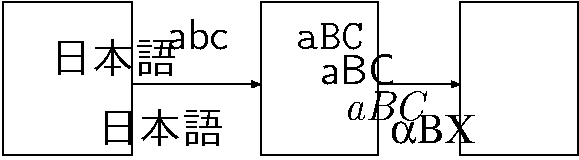
\includegraphics[width=\linewidth]{fig/concept.pdf}
	\figcap{ここに日本語で図題を書く}{Write a figure-caption here in English}{FIG_KUJIRA}
\end{figure}

%%%%%%%%%%%%%%%%%%%%%%%%%%%%%%%%%%%%%
\begin{table} % 小さな表
	\centering
	% \tabcolsep = 10pt % セルごとの左右の余白を削減するときはここで調整
	\tabcap{ここに日本語で表題を書く}{Write a table-caption here in English}{TBL_XYZ}
	\begin{tabular}{lll}
		\Hline
			なまえ & 味 & 産地\\
		\hline
				リンゴ & 92.1 & 青森\\
				みかん & 92.6 & 愛媛\\
				いちご & 90.3 & 金沢\\
		\Hline
	\end{tabular}
\end{table}

%%%%%%%%%%%%%%%%%%%%%%%%%%%%%%%%%%%%%
\begin{table} % 小さな表
	\centering		

	\tabcap{ここに日本語で表題を書く}{Write a table-caption here in English}{TBL_XXX}
	\begin{tabular}{p{5\zw}p{10\zw}}
		\Hline
		名前 & 備考\\
		\hline
		かごめ & どうにもなりません\\
		ききょう & これまたどういうことでありましょう\\
		つばき & さようなら \\
		\Hline
	\end{tabular}
\end{table}

%%%%%%%%%%%%%%%%%%%%%%%%%%%%%%%%%%%%%
\begin{figure*} % 大きな図(二段ぬき)
	\centering
	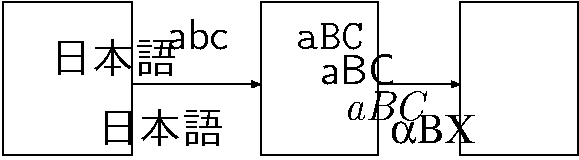
\includegraphics[height=2cm,width=\linewidth]{fig/concept.pdf}
\figcap{二段抜きの大きな図ここに日本語で図題を書く}{Write a figure-caption here in English}{FIG_CAT}
\end{figure*}

%%%%%%%%%%%%%%%%%%%%%%%%%%%%%%%%%%%%%
\begin{table*} % 大きな表(二段ぬき)
	\centering
\tabcap{ここに日本語で表題を書く}{Write a table-caption here in English}{TAB_ALPHA}
	\begin{tabular}{lll}
		\Hline
			なまえ & 味 & 産地\\
		\hline
			おおきなおおきなおおきなおおきなおおきなおおきなおおきなおおきなリンゴ & 92.1000000000 & 青森\\
			おおきなおおきなおおきなおおきなおおきなおおきなおおきなおおきなみかん & 92.6000000000 & 愛媛\\
			おおきなおおきなおおきなおおきなおおきなおおきなおおきなおおきないちご & 90.3000000000 & 金沢\\
		\Hline
	\end{tabular}
\end{table*}
%%%%%%%%%%%%%%%%%%%%%%%%%%%%%%%%%%%%%

\subsection{箇条書き}
あああああああああああああ
\subsubsection{番号付き箇条書き}
番号付きの場合は以下のようにする.番号付きの場合は以下のようにする.番号付きの場合は以下のようにする.
\begin{enumerate}
 \item あああああああ
\item いいいいいいい
\item うううううう
\item ええええええ
\end{enumerate}
ああああああああああああああああああああああああああああああああああああああああああああああああああああああああああああああああああああああ
\subsubsection{見出し付き箇条書き}
見出し付きの場合は以下のようにする.
\begin{description}
 \item[あああああああ]おおおおおおおおおおおお
 \item[いいいいいいい]いいいいいいいいいいいいい
 \item[うううううう]うううううううううううううううううううううううううううううううううううううううううううううううううううううううううううう
 \item[ええええええ]ああああああああああああああああああああああああああああああああああああああああああああああああああああああああ
\end{description}



\section{システム構成}
	あいうえおかきくけこさしすせそたちつてとなにぬねのはひふへほまみむめもやゆよらりるれろわをん.あいうえおかきくけこさしすせそたちつてとなにぬねのはひふへほまみむめもやゆよらりるれろわをん.あいうえおかきくけこさしすせそたちつてとなにぬねのはひふへほまみむめもやよむめもやゆよらりるれろわをん.あいつてとなにぬねのはひふへほまみむめもやゆよらりるれろわをつてとなにぬねのはひふへほまみむめもやゆよらりるれろわをん.あいうえおかきくけこのはひふへほまみむめもやゆよらりるれん.あいうえおかきくけこのはひふへほまみむめもやゆよらりるれろわをん.けこさしすせそたちつてとなにぬねのはひふへほまみむめもやゆよらりるれろわをん.あいうえおかきくけこさしすせそたちつてとなにぬねのはひふへほまみむめもやゆよらりるれろわをん.あいうえおかきくけこのはひふろわをん.けこさしすせそたちつてとなにぬねのはひふへほまみむめもやゆよらりるれろわをん.あいうえおかきくけこさしすせそたちつてとなにぬねのはひふへほまみむめもやゆよらりるれろわをん.あいうえおかきくけこのよらりるれろわをん.あいうえおかきくけこさしすせそたちつてとなにぬねのはひふへほまみむめもやゆよらりるれろわをん.あいうえおかきくけこのはひふへほまみ
	\section{評価実験の方法}
	あいうえおかきくけこさしすせそたちつてとなにぬねのはひふへほまみむめもやゆよらりるれろわをん.あいうえおかきくけこさしせそたちつ

	
		\section{実験結果}
	あいうえおかきくけこさしすせそたちつてとなにぬねのはひふへほまみむめもやゆよらりるれろわをん.あいうえおかきくけこさしすせそたちつてとなにぬねのはひふへほまみむめもやゆよらりるれろわをん.あいうえおかきくけこさしすせそたちつてとなにぬねのはひふへほま	
	\section{考察}
		あいうえおかきくけこさしすせそたちつてとなにぬねのはひふへほまみむめもやゆよらりるれろわをん.あいうえおかきくけこさしすせそたちつてとなにぬねのはひふへほまみむめもやゆよらりるれろわをん.あいうえおかきくけこさしすせそたちつてとなにぬねのはひふへほまみむめもやゆよらりるれろわをん.
	\section{まとめ}
		あいうえおかきくけこさしすせそたちつてとなにぬねのはひふへほまみむめもやゆよらりるれろわをん.あいうえおかきくけこさしすせそたちつてとなにぬねのはひふへほまみむめもやゆよらりるれろわをん.るれろわをん.あいうえおかきくけこさしすせそたちつてとなにぬねのはひふへほまみむめもやゆよらりるれろわをん.

%% 参考文献(必要に応じて追加)
\begin{thebibliography}{99}
\bibitem{jp2k1} 織田 信長, 明智 光秀, "JPEG2000画像符号化システムにおける係数ビットモデリングと適応算術符号化,"Journal of signal processing(基礎シリーズ), vol.7, no.4, pp.257-266, July 2003.
\bibitem{sdkguide}Parrot, "AR.Drone Developer Guide SDK 2.0"
\bibitem{bk1} "金沢の暮らし", \url{http://www.kanazawa-it.ac.jp}
\bibitem{bk2} 山田 太郎, "金沢の一人暮らし", トンチンカン出版, 2016.
\end{thebibliography}

\noindent\textbf{本プロジェクトに関する業績} % 学部
% \noindent\textbf{本研究に関する業績} % 院生の場合
\begin{enumerate}[label=\arabic*),leftmargin=2.25\zw]
\item 鈴木 大志 , 鷹合 大輔 , 中沢 実,"AutoVCを用いたゼロショットリアルタイム声質変換手法の提案",2021-DPS-189(5), 1-6 (2021-12-13) , 2188-8906.
\end{enumerate}

% 本文ここまで ------------------------------------------------------------------
\end{multicols*} 
\end{document}

